\documentclass{article}
\usepackage{graphicx}
\usepackage{float}

\begin{document}

\title{CS181 Spring 2016 Practical 3: Predicting Music Tastes | Team EXT3}
\author{Robert J. Johnson | Dinesh Malav | Matthew McKenna}


\maketitle

\begin{abstract}
We attempted to implement unsupervised learning algorithms to predict how often a user would listen to a new song based on his or her's past listening habits. Given data on approximately 233,000 unique users and 2000 unique artists we attempted to fit a model to make predictions for roughly 4.1 million user/artist pairs. The only successful implementation that we were able to create was an implementation of KNN in R; however, this was only able to work on subsets of size 10,000. 
\end{abstract}
\section{Technical Approach}
Essentially, we were tasked with predicting behavior based on previous actions of a user. For the scope of the practical, we did not focus on demographic data about specific users, which likely could have improved and made more robust any models that we were using. There was also a decision not to use any additional information about the artists themselves, such as genre, popularity, and other descriptive factors. In essence, the number of listens were thought of as almost a rating of sorts. We viewed the problem abstractly, positing that a user would behave in a manner similar to other users. If User A listened to Artist A a similar number of times as User B did, then we can intuitively conclude that they would listen to Artist B a similar amount of times.\\\\
In practice however, there are other factors in play. For example, User A and User B may both love rap music. But, User A does not like classical music, whereas User B does in fact enjoy classical music. The reasons behind this may be arbitrary, but a overly simple model such as basing predictions off of mean or median listening times will not help us in predicting the listening habits. Therefore, we chose to attempt to implement the following algorithms.\\\\
These were the approaches were used for this study.\\\\
K-Nearest Neighbors: This technique is the same as just a simple KNN model. Simply put, we want to know which other users are closest to a given user in feature space, and what are the the listening patterns of the similar users.\\\\
Matrix Factorization: Matrix factorization allows us to predict the similarities between users, and in doing so we potentially could unearth latent features in the data system that would allow us to better predict the number of listens.\\\\
User-Based Collaborative Filtering: This brand of collaborative filtering essentially creates a matrix the size of len(users) X len(artists) and algorithmically tries to determine the missing fields. Users that have similar listening patterns will be compared to each other, and this allows us to make predictions.\\\\
Item-Item Collaborative Filtering: The main benefit of this approach is that instead of storing information on similarities between users we can instead store similarities between the artists. This results in a len(artists) X len(artists) sized matrix that is much smaller than a matrix storing information regarding the users. The similarity between two artists can be calculated using different formulas such as a Cosine Similarity or a Pearson Similarity. Additional comparisons can be made using means and medians.\\\\
\section{Results}
Ultimately, we were unable to create a prediction set for the test data. This was largely due to time and computing constraints. Every algorithm that we attempted to implement took hours to run on the Macbook Airs used by the group members. We were unable to find a method that would run in a computationally efficient manner in either Python or R. The closest that our team was able to get was an implementation of KNN in R that was functional, but could not handle the entire data set. Only 10,000 data points were able to be ran at a time. This implementation used the demographic (sex, age, country) in the training dataset to predict the number of plays.  Included below is a histogram of the Prediction Error using the implementation in R. \\\\ 
\begin{center}
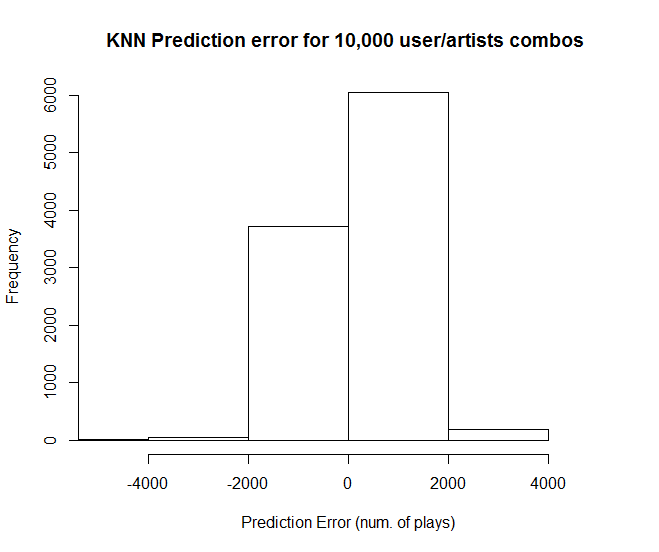
\includegraphics[width=10cm]{pred_diff.png}
\end{center}
\section{Discussion}

Obviously, for further analysis we will either need to come up with better algorithms or increase our computational power. With more time, we would have liked to implement some ensemble methods, such as those utilized in the now-infamous Netflix Prize. Actual, real-life implementations of classifier and recommendation systems use different calculations from different algorithms and aggregate them together to produce accurate results. Complicated techniques using NoSQL databasing and processes distributed across multiple high-powered servers allow these computations to be ran at speeds that we were not able to approach using our personal set-ups.\\\\
All code for this project can be found at: $$https://github.com/HarvardCS181Practical2016$$.





\end{document}